\chapter{Optimal and Robust Control System} \label{ch:optimalrobustcs}

In a typical optimal control problem, a cost function that minimizes regulation error, control signal energy, etc., is defined. Such control that minimizes the cost function is calculated. In a typical robust control problem, stochastic disturbance is introduced into the model, and such control signal that minimizes the average or worst effect of the disturbance is calculated. More details are introduced in this chapter.

The key to optimal and robust control is to solve the optimization problem using variety of mathematical tools.

\section{Static Optimization}

Assume static model where there is no dynamic response. Find the signal $u$ that minimizes the static cost function $L(u)$ (or $L$ for simplicity). Notice that $u\in\mathbb{R}^m$ and $L$ a scalar. 

\subsection{Optimization without Constraint}

Using Taylor series expansion, An increment of $L$ can be formulated as follows.
\begin{eqnarray}
	dL &=& L_u^Tdu + \dfrac{1}{2}du^TL_{uu}du + \ldots \nonumber
\end{eqnarray}
where
\begin{eqnarray}
	L_u &=& \dfrac{\partial L}{\partial u} \in \mathbb{R}^m \nonumber \\
	L_{uu} &=& \dfrac{\partial^2 L}{\partial u^2} \in \mathbb{R}^{m\times m}
\end{eqnarray}
about a particular choice of $u$. A (local) minimum of $L$ is achieved under the following conditions. Firstly,
\begin{eqnarray}
	L_u &=& 0 \nonumber \\
	dL &\geq& 0 \label{eq:optimalrobustcs:dlispositive}
\end{eqnarray}
which indicates that it is a critical point (also known as stationary point) at the choice of $u$, and $L$ increases around that critical point. Equation \eqref{eq:optimalrobustcs:dlispositive} is equivalent to
\begin{eqnarray}
	L_{uu} &>& 0 \nonumber
\end{eqnarray}
a positive definite matrix.

Consider the following example.
\begin{shortbox}
\Boxhead{A Quadratic Surface Example}

Let
\begin{eqnarray}
	L &=& \dfrac{1}{2}u^TQu + Su \label{eq:optimalrobustcs:quadraticsurfacecostfunc1} \\
	&=& \dfrac{1}{2}u^T\left[\begin{array}{cc}
		q_{11} & q_{12} \\
		q_{21} & q_{22}
	\end{array}\right]u + \left[\begin{array}{cc}
	s_1 & s_2
	\end{array}\right]u \label{eq:optimalrobustcs:quadraticsurfacecostfunc2}
\end{eqnarray}
Find $u$ at the critical point, and discuss whether it is a maximum, minimum or other.

\end{shortbox}

From \eqref{eq:optimalrobustcs:quadraticsurfacecostfunc1} and \eqref{eq:optimalrobustcs:quadraticsurfacecostfunc2},
\begin{eqnarray}
	L_u &=& Qu + S \nonumber \\
	L_{uu} &=& Q \nonumber 
\end{eqnarray}
At critical point $L_u=0$,
\begin{eqnarray}
	u^* &=& -Q^{-1}S \nonumber
\end{eqnarray}
where $u^*$ denotes the critical point. Whether this critical point is a maximum, minimum, or other cases depends on $L_{uu}$. 
\begin{itemize}
	\item If $L_{uu}>0$, i.e. $Q$ is positive definite, the critical point is a minimum.
	\item If $L_{uu}<0$, i.e. $Q$ is negative definite, the critical point is a maximum.
	\item Otherwise, \begin{itemize}
		\item If $|L_{uu}|<0$, i.e. $q_{11}q_{22}-q_{12}q_{21}<0$, the critical point is a saddle point.
		\item If $|L_{uu}|=0$, the critical point is a singular point and more information is required to determine the shape at the critical point.
	\end{itemize}
\end{itemize}

\subsection{Optimization with Equality Constraint}

Consider the optimization with equality constraint as follows.
\begin{eqnarray}
	\textup{minimize} && L(u) \label{eq:optimalrobustcs:equalityconsfunc} \\
	\textup{s.t.} && f(u) = 0 \label{eq:optimalrobustcs:equalityconstraint}
\end{eqnarray}
where $u\in\mathbb{R}^m$ and $f(u)\in\mathbb{R}^n$, and without losing generality we assume that $n<m$ (otherwise $u$ can be solved from $f(u)=0$).

\vspace{0.1in}
\noindent \textbf{Intuitive Explanation}
\vspace{0.1in}

It is obvious that the solution to \eqref{eq:optimalrobustcs:equalityconsfunc} would not be necessarily at $L_u=0$. As a matter of fact, at any point of $u$ satisfying $f(u)=0$, it is not necessary that $L_u=0$. This is demonstrated by Fig. \ref{fig:optimalrobustcs:opt_equalityconstraint_contour},
\begin{figure}
	\centering
	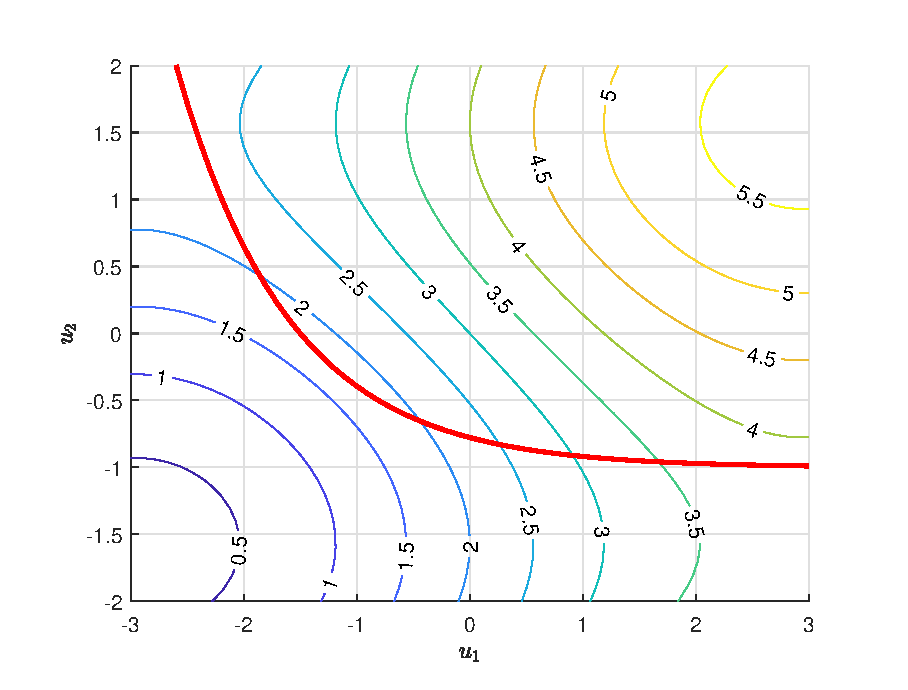
\includegraphics[width=300pt]{chapters/ch-optimal-robust-control-system/figures/opt_equalityconstraint_contour.eps}
	\caption{Static optimization with equality constraint demonstration.} \label{fig:optimalrobustcs:opt_equalityconstraint_contour}
\end{figure}
where $L(u)$ is given by the contour (assuming $u\in\mathbb{R}^2$ in this demonstration), and $f(u)=0$ the red solid line.

The critical point of \eqref{eq:optimalrobustcs:equalityconsfunc} can be found as follows. Consider a necessary condition for the critical point. At the critical point, $L_u = dL / du$ is not necessary zero, and neither is $dL$ for all random chosen $du$. However, $dL$ should be zero with respect to $du$ when $df$ is zero, i.e. (consider only the first-order Taylor expansion for now),
\begin{eqnarray}
	&& dL = L_u^Tdu = 0 \label{eq:optimalrobustcs:equalitycritical1} \\
	\textit{s.t.} && df = f_udu = 0 \label{eq:optimalrobustcs:equalitycritical2}
\end{eqnarray}
or equivalently
\begin{eqnarray}
	\left[\begin{array}{c}
		dL_{\color{red} 1\times 1} \\ df_{\color{red} n\times 1}
	\end{array}\right]_{\color{red} (n+1)\times 1} = \left[\begin{array}{c}
	{L_u^T}_{\color{red} 1\times m} \\ {f_u}_{\color{red} n\times m} 
	\end{array}\right]_{\color{red} (n+1)\times m}du_{\color{red} m\times 1} = 0 \label{eq:optimalrobustcs:equalitycritical3}
\end{eqnarray}
For reading convenience, the dimensions of the matrices are given in red color.

As a necessary condition, given a critical point, we should be able to solve \eqref{eq:optimalrobustcs:equalitycritical2} for a linear space of $du$, and make sure that such $du$ satisfies \eqref{eq:optimalrobustcs:equalitycritical1}. With that been said, the coefficient matrix $[L_u^T; f_u]$ in \eqref{eq:optimalrobustcs:equalitycritical3} should have rank of at most $n$ so that the last $n$ rows alone can be used to find $du$ then substitute it to the first row for verification. Therefore, \eqref{eq:optimalrobustcs:equalitycritical3} can be re-written as follows.
\begin{eqnarray}
	\left[\begin{array}{cc}
		1 & \lambda^T
	\end{array}\right] \left[\begin{array}{c}
	L_u^T \\ f_u
	\end{array}\right] &=& 0 \nonumber \\
	L_u^T + \lambda^Tf_u &=& 0 \label{eq:optimalrobustcs:equalitycritical4}
\end{eqnarray}
where $\lambda \in \mathbb{R}^n$ is known as the Lagrange multipliers, and \eqref{eq:optimalrobustcs:equalitycritical4} a set of $m$ equations being a simplified part of Karush–Kuhn–Tucker (KKT) conditions which will be introduced in more details later.

Equation \eqref{eq:optimalrobustcs:equalitycritical4} can also be interpreted graphically. It suggest that the gradient of $L(u)$ and $f(u)$ should be parallel at the critical point by a factor of $\lambda$. This is shown by Fig. \ref{fig:optimalrobustcs:opt_equalityconstraint_graphical}. At the critical point denoted by the red dot, the red solid line $f(u)=0$ tangents the contour $L(u)$ indicated by the red dashed line. The gradient of both $f_u=\nabla f$ and $L_u=\nabla L$ should be perpendicular to the tangent aligning with the red arrows, hence they are parallel.
\begin{figure}
	\centering
	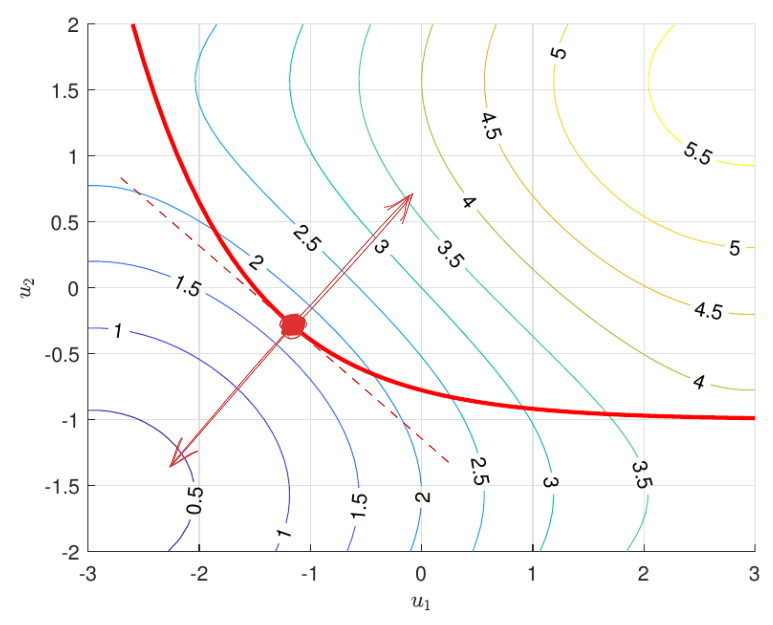
\includegraphics[width=300pt]{chapters/ch-optimal-robust-control-system/figures/opt_equalityconstraint_graphical.png}
	\caption{Graphical explanation to \eqref{eq:optimalrobustcs:equalitycritical4}.} \label{fig:optimalrobustcs:opt_equalityconstraint_graphical}
\end{figure}

Equation \eqref{eq:optimalrobustcs:equalitycritical4} together with \eqref{eq:optimalrobustcs:equalityconstraint} forms the necessary condition for the solution of the optimization problem.

\vspace{0.1in}
\noindent \textbf{Lagrangian Function}
\vspace{0.1in}

The necessary condition can also be derived using Lagrangian function as follows. Lagrangian function is a very useful tool in solving optimization problem with different types of constraints. Notice that Lagrangian function in some context may also be called Hamiltonian function. They are very similar mathematically, and mostly differ in the context of usage.
\begin{eqnarray}
	\mathcal{L}(u, \lambda) &=& L(u) + \lambda^Tf(u) \label{eq:optimalrobustcs:lagarangianequality} \\
	&=& L(u) + \sum_{i=1}^{n}\lambda_if_i(u) \nonumber
\end{eqnarray}
and \eqref{eq:optimalrobustcs:equalityconstraint}, \eqref{eq:optimalrobustcs:equalitycritical4} can be represented by
\begin{eqnarray}
	\dfrac{\partial \mathcal{L}}{\partial \lambda} &=& 0 \nonumber \\
	\dfrac{\partial \mathcal{L}}{\partial u} &=& 0 \nonumber
\end{eqnarray}
respectively.

It is difficult to find the critical point for the original problem with equality constraint. However, by introducing Lagrangian function \eqref{eq:optimalrobustcs:lagarangianequality}, the problem becomes finding critical point for Lagrangian function without constraint. This is made possible due to the introduction of Lagrange multipliers $\lambda$ that adds some flexibility to the equation, making it contain the information of equality constraint in a ``disguised'' manner.

\vspace{0.1in}
\noindent \textbf{Sufficient Condition}
\vspace{0.1in}

The necessary condition helps to pick up the possible candidates that may be a local minimum of the optimization problem. To verify that the critical point is indeed a local minimum, check the second-order derivative $\partial^2 L / \partial u^2$ of the critical point.

Consider the following example.
\begin{shortbox}
\Boxhead{A Quadratic Surface Example with Linear Equality Constraint}

Let
\begin{eqnarray}
	L(x, u) &=& \dfrac{1}{2}x^TQx + \dfrac{1}{2}u^TRu \nonumber \\
	\textup{s.t.} \nonumber \\ f(x, u) &=& x + Bu + c \nonumber \\ &=& 0 \nonumber
\end{eqnarray}
Find $u$ at the critical point, and discuss whether it is a minimum.

\end{shortbox}






\subsection{Optimization with Equality and Inequality Constraints}

\section{Discrete LQR}

\section{Continuous LQR}

\section{LQR for Tracking}

\section{LQG}

\section{$H_2$ and $H_\infty$ Control} 